%%%%%%%%%%%%%%%%%%%%%%%%%%%%%%%%%%%%%%%%%%%%%%%%%%%%%%%%%%%%%%%%%%%%%%%%%%%%%%%%%%%%%%%%%%%%%%%%%%%%%%%%%%%%%%%%
\subsection{Informal description}

An interactive entity is an entity that can interact with other entities by exchanging information in the form of data flows. A human being is an interactive entity, a controllable embedded system is an interactive entity, a human-machine interface is an interactive entity. They are all able to exchange information in different directions, using different means (eyes, hands, bus, network, screen, keyboard...)


A first important thing to notice is that, in order to interact, two interactive entities must establish a data flow, by matching an entity's input to another entity's output.

LIDL is a language that allows to specify interactive entities, called interactors. A LIDL interactor is described through two different aspect: interfaces and interactions. Interfaces are the description of the data flows between the interactor and other interactive entities. Interactions are the description of the link between input data flows and output data flows.

As a first short example, Listing~\ref{buttoninterface} is a piece of LIDL code that defines the interface associated with a button interactor. This definition specifies that a button has a title, which is a text output to the user, and it can receive clicks, which are activation signals coming from the user.

\begin{lstlisting}[caption=Interface of the speed controller,label=buttoninterface]
interface Button is
	{
		title: text out,
		click: activation in	
	}
\end{lstlisting}

Listing~\ref{buttoninteraction} is a piece of LIDL code that defines the interaction associated with a button interactor. It specifies a pattern of use \code{(Button(...)with title(...)triggerring(...))}, along with the interfaces associated with arguments, the interface of the interaction itself \code{Button}, and an interaction expression which is the definition of this interaction.


\begin{lstlisting}[caption=Interaction of a button,label=buttoninteraction]
interaction 
	(Button (status: activation in) 
	with title (theTitle: text in) 
	triggering (onClick: activation out))
implementing
	Button
is
	(bind(this) : (when (status) : (all
			((this.title)=(theTitle))
			((onClick)=(this.click))
	)))
\end{lstlisting}


Listing~\ref{buttonuse} is an instantiation of the interaction defined in Listing~\ref{buttoninteraction}. It creates a Button whose status is always \code{active}, which has the title \code{"Ok"}, and which, when clicked, activates another interaction called \code{Beep}. 

\begin{lstlisting}[caption=Usage of a button,label=buttonuse]
(myButton) = (Button(active) with title ("Ok") triggering (beep))
\end{lstlisting}








%%%%%%%%%%%%%%%%%%%%%%%%%%%%%%%%%%%%%%%%%%%%%%%%%%%%%%%%%%%%%%%%%%%%%%%%%%%%%%%%%%%%%%%%%%%%%%%%%%%%%%%%%%%%%%%%
\subsection{Syntax}

LIDL is very general, and so is its syntax. The syntax use lots of parentheses, which is a solution to two contradictory requirements: \textbf{REQ2} and \textbf{REQ3}. Interaction expressions are used to compose interactions in order to form more complex interaction patterns. This grammar is very simple, here is the extended Backus Naur form (EBNF) of the interaction grammar of LIDL:

\begin{figure}
\begin{grammar}
<interaction> ::= `(' <element>* `)'

<element> ::= <interaction>
 \alt <word>
 
<word> ::= ? anything except parentheses ?
	
\end{grammar}
\caption{Expression grammar of LIDL}
\label{fig-expr-grammar}
\end{figure}



Said simply, an interaction is expressed as a sentence between parentheses. The interactions it refers to are also between parentheses. LIDL syntax is made in such a way that every parentheses pair \code{(...)} is an interaction, and reciprocally. 

The interaction expression in Listing~\ref{buttoninteraction} is composed of several interactions, each between parentheses. Figure~\ref{fig-expr-tree} shows the expression tree associated with this expression.


\begin{figure}
\begin{center}
\includegraphics[width=\columnwidth,page=12]{drawings.pdf}
\end{center}
\caption{The expression tree associated with Listing~\ref{buttoninteraction}}
\label{fig-expr-tree}
\end{figure}


%%%%%%%%%%%%%%%%%%%%%%%%%%%%%%%%%%%%%%%%%%%%%%%%%%%%%%%%%%%%%%%%%%%%%%%%%%%%%%%%%%%%%%%%%%%%%%%%%%%%%%%%%%%%%%%%
\subsection{Synchronous execution}


LIDL systems are synchronous. This means that interactions are evaluated at discrete points in time, all at once. The interaction expression defining a system is evaluated at discrete points in time, called steps. Every expression of this composed expression will be evaluated at every step. 

Synchronous execution avoids spaghetti behaviours. The state of the system is explicitly defined for each execution step. This makes reasoning about code much simpler, verification is much easier than with other asynchronous approaches.

Figure~\ref{fig-sync-exec} shows the synchronous execution of a LIDL system. TODO : talk about the transition function here


\begin{figure*}
\begin{center}
\includegraphics[width=\textwidth,page=17]{drawings.pdf}
\end{center}
\caption{Execution of a LIDL System with $x$ input variables $\{i^1 \hdots i^x\}$, $y$ state variables $\{s^1 \hdots s^y\}$, and $z$ output variables $\{o^1 \hdots o^z\}$. The transition function is named $f$, its domain is in blue, its codomain is in red.}
\label{fig-sync-exec}
\end{figure*}

%%%%%%%%%%%%%%%%%%%%%%%%%%%%%%%%%%%%%%%%%%%%%%%%%%%%%%%%%%%%%%%%%%%%%%%%%%%%%%%%%%%%%%%%%%%%%%%%%%%%%%%%%%%%%%%%
\subsection{Activation}

One of the contribution of the LIDL language is the built-in notion of activation. Each piece of data in LIDL is attached to an activation. This notion is some kind of abstraction over other similar features like \code{null} values.

An interaction's activation represents the fact that the interaction exists and is active at a point in time, or not. For example, if an interaction represents an event, then it will only be activated when the event happens. As another example, the assignment interaction \code{$=$} is only effective when it is active. If an interaction's value is not defined anywhere, then its activation is false.




In previous approaches, and in some other languages, a difference is made between events and flows, which are considered as two different first-class entities. Some languages only allow one of those. In these approaches, events represent data defined at discrete points in time, while flows represent data defined on continuous time intervals. But when we think about it, the only difference between an event and a flow lies in the domain. For events this set is discrete. For flows this set is continuous.

The logical conclusion of this remark is that the merger of these two concepts needs to include the indicator function of the domain. This indicator function is the activation.

\subsection{Flow direction}

Reciprocity (in matches out)

%%%%%%%%%%%%%%%%%%%%%%%%%%%%%%%%%%%%%%%%%%%%%%%%%%%%%%%%%%%%%%%%%%%%%%%%%%%%%%%%%%%%%%%%%%%%%%%%%%%%%%%%%%%%%%%%
\subsection{Formal description}


\subsubsection{Identifier}

\begin{definition}[Identifier]
$\mathbb{I}$ is the set of all possible identifiers. An identifier $i \in \mathbb{I}$ is noted $i=\codemath{foo}$
\end{definition}

\noindent
Each interaction instance has an identifier associated with it. The identifier associated with an interaction is the LIDL code of this interaction, with white spaces removed. For example the interaction noted \code{(when (click) : (beep) )} in LIDL is associated to the identifier
$\codemath{(when(click):(beep))}$.





\subsubsection{LIDL system}



The basic notion is the interactive component named \code{interaction} which produces output and new current internal state flows from input and previous  internal state flows. Each instance of an interaction is associated with an identifier.




\begin{definition}[LIDL System]
$\mathcal{P}(\mathbb{I})$ is the set of all possible LIDL systems.
\end{definition}

A LIDL system is a composition of interactions that defines a more complex interaction. 

Homoiconicity
le fait qu’un programme puisse se représenter dans les structures de données du langage lui-même 






\begin{definition}[Value]
$\mathbb{V} = \{\bot\}\cup\{\top\}\cup\mathbb{B}\cup\mathbb{R}\cup\mathbb{T}$ is the set of all atomic values of the LIDL language, where $\mathbb{B}$ the booleans, $\mathbb{R}$ the set of real numbers, $\mathbb{T}$ the set of all possible texts. The set of all possible values of the LIDL language, including composed values is $\mathbb{V}^*$.
\end{definition}

\noindent
There are 4 base data types in LIDL:
\begin{itemize}
	\item \code{activation}, whose value set is $\{\top\}$, the active value.
	\item \code{boolean}, whose value set is $ \mathbb{B} =  \{true, false\}  $
	\item \code{number}, whose value set is $ \mathbb{R} $, the real numbers
 	\item \code{text}, whose value set is $\mathbb{T}$, the set of all possible texts
\end{itemize}

\noindent
Each 



\begin{definition}[Memory]
$\mathbb{M} = \mathbb{V}^\mathbb{I}$ is the set of all possible memories of a LIDL system. A memory $m \in \mathbb{M}$ is a function noted $m:\mathbb{I}\rightarrow\mathbb{V}$.
\end{definition}


\begin{definition}[Execution]
$\mathbb{E} = \mathbb{M}^\mathbb{N}$ is the set of all possible executions of a LIDL system, where $\mathbb{N}$ is the set of natural numbers. An execution is a function noted $e:\mathbb{N}\rightarrow\mathbb{I}\rightarrow\mathbb{V}$
\end{definition}

\begin{definition}[Valuation]
$\codemath{foo}_n^e$ denotes the value associated to the identifier $\codemath{foo}$, in the $n^{th}$ memory of an execution $e$. 
\end{definition}


\[\forall n < 0 \quad \forall \codemath{x} \in \mathbb{I} \quad \codemath{x}_n^e = \bot\]

\[\forall n \geq 0 \quad \forall \codemath{x} \in \mathbb{I} \quad \exists f \quad \codemath{x}_n^e = f()\]

In the following tables, values on the left side of the vertical bar are the ones which have to be computed beforehand, so that values on the right side of the vertical bar can be computed. Values noted as letters such as $x$ are supposed to be different from $\bot$.

Here is an example, where input1 and input2 are input values, and ouput1 and output2 are output values. The example reads like this : on execution step $n$ when input1=a and input2=b, then output1=x and output2=y...

\begin{center}
\begin{tabular}{cc|cc}
  $\codemath{(input1)}_n^e$ & $\codemath{(input2)}_n^e$ & $\codemath{(output1)}_n^e$ & $\codemath{(output2)}_n^e$ \\
  \hline
  $a$&$b$&$x$&$y$ 
\end{tabular}
\end{center}




Affectation


\begin{center}
\begin{tabular}{cc|c}
  $\codemath{((a)=(b))}_n^e$ & $\codemath{(b)}_n^e$ & $\codemath{(a)}_n^e$ \\
  \hline
  $\bot$&$\bot$ &$\bot$ \\
  $\bot$& $b$&$\bot$ \\
  $\top$& $\bot$&$\bot$ \\
  $\top$& $b$&$b$ \\
\end{tabular}
\end{center}



All

\begin{center}
\begin{tabular}{c|cc}
  $\codemath{(all(a)(b))}_n^e$ & $\codemath{(a)}_n^e$ & $\codemath{(b)}_n^e$ \\
  \hline
  $\bot$&$\bot$ &$\bot$ \\
  $\top$& $\top$&$\top$ \\
\end{tabular}
\end{center}


Either

\begin{center}
\begin{tabular}{c|cc}
  $\codemath{(either(a)(b))}_n^e$ & $\codemath{(a)}_n^e$ & $\codemath{(b)}_n^e$ \\
  \hline
  $\bot$& $\bot$ &$\bot$ \\
  $\top$& $\top / \bot$& $\bot / \top$ \\
\end{tabular}
\end{center}

Always

\begin{center}
\begin{tabular}{c|c}
  $\codemath{(always(a))}_n^e$ & $\codemath{(a)}_n^e$ \\
  \hline
  $\bot$& $\top$  \\
  $\top$& $\top$ \\
\end{tabular}
\end{center}

Previous

\begin{center}
\begin{tabular}{|c}
    $\codemath{(previous(a))}_n^e$ \\
  \hline
  $\codemath{(a)}_{n-1}^e$
\end{tabular}
\end{center}

Arithmetic operators

\begin{center}
\begin{tabular}{cc|c}
  $\codemath{(a)}_n^e$ & $\codemath{(b)}_n^e$ & $\codemath{((a)+(b))}_n^e$ \\
  \hline
  $\bot$& $\bot$ & $\bot$ \\
  $\bot$& $b$ & $\bot$ \\
   $a$& $\bot$ & $\bot$ \\
   $a$& $b$ & $a+b$ 
\end{tabular}
\end{center}


If then else

\begin{center}
\begin{tabular}{ccc|c}
  $\codemath{(a)}_n^e$ &$\codemath{(b)}_n^e$ & $\codemath{(c)}_n^e$  & $\codemath{(if(a)then(b)else(c))}_n^e$ \\
  \hline
$\bot$ &$\bot$ &$\bot$ &$\bot$ \\
$\bot$ &$\bot$ &$c$ &$\bot$ \\
$\bot$ &$b$ &$\bot$ &$\bot$ \\
$\bot$ &$b$ &$c$ &$\bot$ \\
$true$ &$\bot$ &$\bot$ &$\bot$ \\
$true$ &$\bot$ &$c$ &$\bot$ \\
$true$ &$b$ &$\bot$ &$b$ \\
$true$ &$b$ &$c$ &$b$ \\
$false$ &$\bot$ &$\bot$ &$\bot$ \\
$false$ &$\bot$ &$c$ &$c$ \\
$false$ &$b$ &$\bot$ &$\bot$ \\
$false$ &$b$ &$c$ &$c$ 
\end{tabular}
\end{center}

Init

\begin{center}
\begin{tabular}{|c}
 $\codemath{(init)}_n^e$ \\
  \hline
$\left\{
     \begin{array}{ll}
       \top & \mbox{if} \: n=0 \\
       \bot & \mbox{else}
     \end{array}
     \right. $
\end{tabular}
\end{center}

Constant litterals

\begin{center}
\begin{tabular}{|c}
  $\codemath{("a text")}_n^e$ \\
  \hline
  $\mathrm{``a \: text"}$
\end{tabular}
\end{center}

\begin{center}
\begin{tabular}{|c}
  $\codemath{(1234)}_n^e$ \\
  \hline
  $1234$
\end{tabular}
\end{center}

\begin{center}
\begin{tabular}{|c}
  $\codemath{(true)}_n^e$ \\
  \hline
  $\mathrm{true}$
\end{tabular}
\end{center}

\begin{center}
\begin{tabular}{|c}
  $\codemath{(active)}_n^e$ \\
  \hline
  $\top$
\end{tabular}
\end{center}

\begin{center}
\begin{tabular}{|c}
  $\codemath{(inactive)}_n^e$ \\
  \hline
  $\bot$
\end{tabular}
\end{center}




\subsubsection{Data types and value sets}

\noindent
Basic data types
\[
  \begin{matrix*}[l]
  \mathtt{activation} & = & \{ \bot\} \cup \{ \top\}\\
  \mathtt{boolean} & = & \{ \bot\} \cup \{ true, false\} \\
  \mathtt{number} & = & \{ \bot\} \cup \mathbb{R}\\
  \mathtt{text} & = & \{ \bot\} \cup all\_possible\_texts\\
\end{matrix*}
\]  

\noindent
Compound types (examples)
\[
  \begin{matrix*}[l]
  \mathtt{[number]} & = & \{ \bot\} \cup \bigcup_{n \in \mathbb{N}} \mathtt{number}_n^e \\
  \mathtt{(number,number)} & = & \{ \bot\} \cup ( \mathtt{number} \times \mathtt{number} ) \\
  \mathtt{\{x:number,y:number\}} & = & \{ \bot\} \cup ( \mathtt{number} \times \mathtt{number} ) \\
  \mathtt{|number,boolean|} & = & \mathtt{number} \cup \mathtt{boolean}  \\

\end{matrix*}
\]  


\subsubsection{Lustre examples of some base interactions}

\begin{lstlisting}
node Affect 
	(actX:bool, valX:int, actB:bool, valB:int)
returns 
	(actA:bool, valA:int);
let
	actA = actX and actB;
	valA = valB;
tel
\end{lstlisting}


\begin{lstlisting}
node All
	(actX:bool, valX:int)
returns 
	(actA:bool, valA:int, actB:bool, valB:int);
let
	actA = actX;
	valA = valX;
	actB = actX;
	valB = valX;
tel
\end{lstlisting}


\begin{lstlisting}
node Always
	(actX:bool, valX:int)
returns 
	(actA:bool, valA:int);
let
	actA = true;
	
tel
\end{lstlisting}


\subsubsection{Composition}

LIDL offers \textbf{referential transparency}, which means that composition of interactions is very simple and works by simple substitution. 


\subsection{Formal semantics}
We define the actual behaviors of a LIDL interaction system by using a
semantics of traces that permits to characterize the behaviors of a
LIDL description in terms of execution traces. Intuitively every
behavior of a LIDL interaction systems corresponds to the sequences of
the values each LIDL variable has. These values define a \textit{state} of the
system and a sequence of states defines a behavior of this system. 

\begin{definition}[Memory]
Let $I$ a set of identifiers of LIDL. $V$ is a set of values and
$\bot$ denotes an undefined value. We define $A = \{false,true\}$.
Every function $\sigma : I \rightarrow A \times (V \cup \{\bot\})$ defines a
memory of the LIDL interaction system.
\end{definition}
Every state of a LIDL interaction system is characterized by a
memory that gives a  value $\sigma(id)$ to each $id \in I$. This
value is a pair $(a,v)$ with $ a \in A$ and $v \in (V \cup
\bot)$ : $a$ indicates if $id$ is \textit{active} or not. If not, $v$ is
not significant and stays undefined ($v = \bot$). 
\begin{definition}[Trace]
An execution trace $\Sigma$ is a non empty, finite or infinite,
sequence of memories.
\end{definition} 
Some  identifiers  play a  particular  role  in the  LIDL  interaction
systems.  They are used to denote \textit{activation signals} that are
not valuated.  Their values are in $A \times \{\bot\}$.  By default
$\forall id  \in I,  \sigma(id) = (false,\bot)$.   In other  words, by
default, every value is not  active. To become  active and to  get a
significant data value, a behavior of the LIDL interaction system must be
activated.

\subsubsection{Semantics of LIDL expressions over finite traces}
The value (in $A \times (V \cup \{\bot\})$ of a LIDL expression $E$
over a finite trace $\Sigma = (\sigma_0,\ldots,\sigma_n^e)$ is defined
by induction on the structure of $E$. We denote $\Sigma \vdash E |
(a,v)$ to mean that $E$ has the value $(a,v)$ ($a \in A$ and $v \in  A
\times (V \cup \{\bot\})$) over $\Sigma$. \\
\noindent
\textbf{Constants values.} If k denotes a bool, number or text constant
then $\Sigma \vdash$ (\mbox{k})$ | (true,k)$. A particular activation
constant, $active$ is defined in LIDL such that $\Sigma \vdash (active) | (true, \bot)$.\\
\noindent
\textbf{Variables values.} $(\sigma_0,\ldots,\sigma_n^e) \vdash (x) |
\sigma_n^e(x)$ if $x$ denotes a variable in the language.\\
\noindent
\textbf{Boolean and arithemtic operators.} If $E_1,\ldots,E_m$ denote
expressions in LIDL and $\star$ is a boolean or arithmetic operator
then $$\frac{\Sigma \vdash (E_1) | (a_1,v_1),\ldots,\Sigma \vdash (E_m) |
  (a_m,v_m)}{\Sigma \vdash \star(E_1,\ldots,E_m) |
  (\bigwedge_{i=1}^{m}a_i, \star(v_1,\ldots,v_m))}$$\\
\noindent
\textbf{Operator previous.} If $E$ denotes an expression in LIDL,
$$\sigma_0 \vdash (\mbox{previous}(E)) | (false,\bot)$$
$$\frac{\Sigma
  \vdash (E) | (a,v)}{\Sigma \cdot \sigma \vdash (\mbox{previous}(E)) | (a,v)}$$\\
\noindent
\textbf{Operator isactive.} If $E$ denotes an expression in LIDL,
$$\frac{\Sigma \vdash (E) | (a,v)}{\Sigma \vdash (\mbox{isactive}(E)) | (true, a)}$$\\
\noindent
\textbf{Operator if then else.} If $E_1$ is a boolean expression in
LIDl and if $E_2$ and $E_3$ are expressions in LIDL,
$$\frac{\Sigma \vdash (E_1)|(a_1,v_1),\Sigma \vdash (E_2)|(a_2,v_2),
  \Sigma \vdash (E_3)|(a_3,v_3)}{\Sigma \vdash \mbox{if} (E_1)
  \mbox{then} (E_2) \mbox{else} (E_3) | 
   \left\{
     \begin{array}{ll}
       (false, \bot) & \mbox{if} a_1 = false \\
       (a_2,v_2) & \mbox{if} (a_1,v_1) = (true,true)\\
       (a_3,v_3) & \mbox{if} (a_1,v_1) = (true,false)
     \end{array}
     \right.
}
$$
\subsubsection{Compatibility  of   an  infinite  trace  with   a  LIDL
description} 

Behaviors that  are described by LIDL interactions are  infinite. The
semantics of a LIDL description corresponds to the set of the infinite
execution traces that  are compatible with it. We  note $\Sigma \vdash
D$ the  fact that an  infinite trace  $\Sigma$ is compatible  with the
LIDL description $D$.

An infinite trace denotes a behavior of $D$ if and only if every
finite prefix of $D$ is compatible with $D$ :
$$(\sigma_0,\ldots,\sigma_n^e,\ldots) \vdash D \Longleftrightarrow
\forall n \geq 0 , (\sigma_0,\ldots,\sigma_n^e) \vdash D$$

The compatibility of finite traces with $D$ is defined by the
following rules. A LIDL description is considered as  (and can be
unfold in) a set of elementary interactions, depicted by equations, regardless of its syntactical
structure. LIDL is a declarative language so the order of the equations is unimportant. 

A new identifier $\langle (interaction) \rangle
\in I$ is associated with every elementary interaction $(interaction)$. $\langle (interaction) \rangle$ denotes the activation signals
that trigger $(interaction)$ : $\sigma(\langle (interaction)
\rangle) \in A \times \{\bot\}$.\\
\noindent
\textbf{Compatibility with an equation.} If x is a LIDL identifier, E
is a LIDL expression :
$$\frac{(\sigma_0,\ldots,\sigma_n^e) \vdash \mbox{(E)} | (a,v),
  \sigma_n^e(\mbox{x}) =
  (a,v), \sigma_n^e(\langle \mbox{(x=E)} \rangle) = (true, \bot)}
{(\sigma_0,\ldots,\sigma_n^e) \vdash \mbox{(x = E)}}
$$\\
\noindent
\textbf{Compatibility with composition.} A set of interactions defines
a new interaction. If $int_1$ and $int_2$ are two interactions
$$\frac{\Sigma \vdash (int_1),\Sigma \vdash (int_2) }
{\Sigma \vdash ((int_1) (int_2))}$$\\
\noindent
\textbf{Compatibility with a guarded interaction.} Let G  an activation
identifier in LIDL ($\sigma(\mbox{I}) \in A \times \{\bot\}$) and $int$ 
a LIDL interaction :
%$$\frac{\begin{array}{c}
%(\sigma_0,\ldots,\sigma_n^e) \vdash (\mbox{G}) | (true,\bot),
%\sigma_n^e(\langle (\mbox{when} (\mbox{G}) \mbox{:} (int) ) \rangle) =
%(true, \bot),\\
% (\sigma_0,\ldots,\sigma_n^e) \vdash \langle (int) \rangle |
%(true,\bot)
%\end{array}}
%{(\sigma_0,\ldots,\sigma_n^e) \vdash (\mbox{when} (\mbox{G}) \mbox{:}
%  (int) )} 
%$$
$$\frac{
\begin{array}{c}
(\sigma_n^e(\mbox{G}) =(true,\bot),
\sigma_n^e(\langle (\mbox{when} (\mbox{G}) \mbox{:} (int) ) \rangle) =
(true, \bot),\\
 \sigma_n^e(\langle (int) \rangle) = (true,\bot)
\end{array}
}
{(\sigma_0,\ldots,\sigma_n^e) \vdash (\mbox{when} (\mbox{G}) \mbox{:}
  (int) )} 
$$
